\documentclass[12pt,a4paper]{article}

\usepackage[utf8]{inputenc}
\usepackage[T1]{fontenc}
\usepackage{lmodern}
\usepackage[spanish,es-nodecimaldot]{babel}
\usepackage[a4paper,margin=2.5cm]{geometry}
\usepackage{booktabs}
\usepackage{amsmath}
\usepackage{float}
\usepackage{graphicx}
\usepackage{tabularx}
\usepackage{hyperref}

\hypersetup{
    colorlinks=true,
    linkcolor=black,
    urlcolor=blue,
    pdftitle={Predicción de eventos sísmicos peligrosos en minería subterránea}
}

\title{Predicción de eventos sísmicos peligrosos en minería subterránea mediante técnicas de clasificación supervisada}
\author{Martinez Mauricio Leonel\\DNI: 45.549.925}
\date{2026}

\begin{document}

\maketitle

\section{Introducción}

La minería subterránea puede estar expuesta a eventos sísmicos de alta energía que representan un riesgo para la seguridad de los trabajadores, la infraestructura y la continuidad de las operaciones. Estos eventos pueden producir desprendimientos, daños materiales e interrupciones en la actividad minera.

Este trabajo estudia la aplicación de técnicas de clasificación supervisada sobre registros históricos de actividad sísmica y sismoacústica. El objetivo es analizar si la información registrada durante un turno permite clasificar la ocurrencia de un evento sísmico peligroso en el turno siguiente. El desbalance entre clases hace necesario evaluar la capacidad de detección de la clase peligrosa además de la exactitud global.

\section{Problema, pregunta y objetivos}

La tarea se formula como un problema de clasificación binaria. La etiqueta \texttt{class} toma el valor 0 para un registro no peligroso y el valor 1 para un registro peligroso. La pregunta de investigación es:

\begin{quote}
¿Qué variante de árbol de decisión o Naive Bayes ofrece el mejor equilibrio entre rendimiento global y detección de la clase peligrosa en el conjunto Seismic-Bumps?
\end{quote}

El objetivo general es comparar cuatro variantes de clasificación: árbol de decisión base, Naive Bayes base, árbol de decisión con SMOTE y Naive Bayes con SMOTE. Los objetivos específicos son caracterizar el conjunto de datos, establecer un procedimiento reproducible de validación cruzada, analizar matrices de confusión y comparar exactitud, AUC, precisión, recall y F1 de la clase 1.

\section{Datos y metodología}

\subsection{Conjunto de datos}

Se utilizó el conjunto \textit{Seismic-Bumps}, disponible en el repositorio público UCI Machine Learning Repository. El archivo local es \texttt{seismic-bumps.arff}. Contiene 2.584 instancias, 19 atributos totales, 18 atributos predictivos y la variable objetivo \texttt{class}. En la inspección realizada no se detectaron valores faltantes.

\begin{table}[H]
    \centering
    \caption{Características generales del conjunto de datos.}
    \label{tab:dataset-general}
    \begin{tabular}{ll}
        \toprule
        \textbf{Característica} & \textbf{Descripción} \\
        \midrule
        Nombre & Seismic-Bumps \\
        Instancias & 2.584 \\
        Atributos totales & 19 \\
        Atributos predictivos & 18 \\
        Variable objetivo & \texttt{class} \\
        Formato & ARFF \\
        Valores faltantes & No detectados \\
        \bottomrule
    \end{tabular}
\end{table}

\begin{table}[H]
    \centering
    \caption{Distribución de la variable objetivo.}
    \label{tab:class-distribution}
    \begin{tabular}{lrr}
        \toprule
        \textbf{Clase} & \textbf{Cantidad} & \textbf{Proporción} \\
        \midrule
        No peligrosa (0) & 2.414 & 93,42\% \\
        Peligrosa (1) & 170 & 6,58\% \\
        \midrule
        Total & 2.584 & 100,00\% \\
        \bottomrule
    \end{tabular}
\end{table}

\begin{figure}[H]
    \centering
    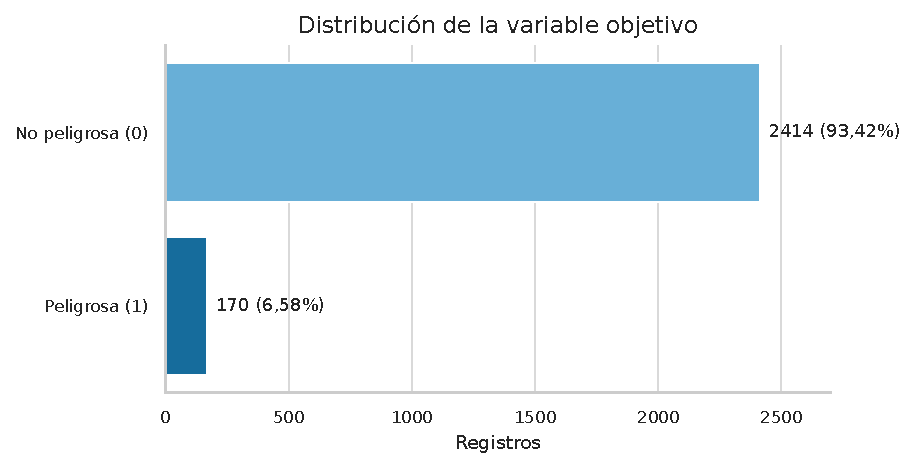
\includegraphics[width=0.78\textwidth]{output/figures/distribucion_clases.pdf}
    \caption{Distribución de las clases del conjunto Seismic-Bumps.}
    \label{fig:class-distribution}
\end{figure}

\subsection{Diseño experimental}

Todos los valores empíricos de este trabajo fueron obtenidos en Altair AI Studio mediante validación cruzada estratificada de 10 particiones. En las variantes con SMOTE, el sobremuestreo se aplicó exclusivamente sobre los datos de entrenamiento de cada partición. El conjunto de prueba conservó la distribución original de las clases. Este procedimiento evita que las observaciones sintéticas o la información del conjunto de prueba intervengan en el entrenamiento y permite comparar las cuatro variantes bajo la misma partición estratificada.

Las matrices se expresan con filas verdaderas y columnas predichas. Para la clase positiva se utilizaron las definiciones habituales: precisión $=TP/(TP+FP)$, recall $=TP/(TP+FN)$ y F1 como media armónica entre precisión y recall. Se informan los valores del encabezado de AI Studio, con su variabilidad entre particiones, y los valores agregados calculados a partir de la matriz total.

\section{Resultados}

\subsection{Árbol de decisión base}

El árbol de decisión base obtuvo una exactitud de 92,84\% $\pm$ 0,27\% y un AUC de 0,860 $\pm$ 0,041. La matriz total fue:

\begin{table}[H]
    \centering
    \caption{Matriz de confusión del árbol de decisión base.}
    \label{tab:dt-base-matrix}
    \begin{tabular}{lrr}
        \toprule
        & \textbf{Predicha 0} & \textbf{Predicha 1} \\
        \midrule
        \textbf{Verdadera 0} & 2.394 & 20 \\
        \textbf{Verdadera 1} & 165 & 5 \\
        \bottomrule
    \end{tabular}
\end{table}

La variante identifica solo 5 de los 170 casos peligrosos. Sus métricas agregadas de clase 1 son precisión 20,00\%, recall 2,94\% y F1 5,13\%. Por lo tanto, la exactitud alta no representa una detección suficiente de la clase minoritaria.

\subsection{Naive Bayes base}

Naive Bayes base obtuvo una exactitud de 84,75\% $\pm$ 4,31\% y un AUC de 0,761 $\pm$ 0,043. La matriz total fue:

\begin{table}[H]
    \centering
    \caption{Matriz de confusión de Naive Bayes base.}
    \label{tab:nb-base-matrix}
    \begin{tabular}{lrr}
        \toprule
        & \textbf{Predicha 0} & \textbf{Predicha 1} \\
        \midrule
        \textbf{Verdadera 0} & 2.120 & 294 \\
        \textbf{Verdadera 1} & 100 & 70 \\
        \bottomrule
    \end{tabular}
\end{table}

La variante identifica 70 casos peligrosos y alcanza precisión agregada de 19,23\%, recall agregado de 41,18\% y F1 agregado de 26,22\%. Este comportamiento mejora la detección de positivos respecto del árbol base, aunque aumenta las falsas alarmas.

\subsection{Árbol de decisión con SMOTE}

El árbol de decisión con SMOTE obtuvo una exactitud de 81,03\% $\pm$ 4,01\%, con valor agregado de 81,04\%, y un AUC de 0,824 $\pm$ 0,068. La precisión de la clase 1 fue 17,95\% $\pm$ 4,15\% en el encabezado y 17,87\% agregada; el recall fue 52,49\% $\pm$ 16,03\% y 52,35\%, respectivamente; el F1 fue 26,50\% $\pm$ 6,39\% y 26,65\%.

La matriz agregada fue
\[
\begin{bmatrix}
2005 & 409 \\
81 & 89
\end{bmatrix},
\]
por lo que $TN=2005$, $FP=409$, $FN=81$ y $TP=89$.

\begin{table}[H]
    \centering
    \caption{Matriz de confusión del árbol de decisión con SMOTE.}
    \label{tab:dt-smote-matrix}
    \begin{tabular}{lrr}
        \toprule
        & \textbf{Predicha 0} & \textbf{Predicha 1} \\
        \midrule
        \textbf{Verdadera 0} & 2.005 & 409 \\
        \textbf{Verdadera 1} & 81 & 89 \\
        \bottomrule
    \end{tabular}
\end{table}

\subsection{Naive Bayes con SMOTE}

Naive Bayes con SMOTE obtuvo una exactitud de 69,94\% $\pm$ 17,58\%, con valor agregado de 69,93\%, y un AUC de 0,748 $\pm$ 0,034. La precisión de la clase 1 fue 15,24\% $\pm$ 3,58\% en el encabezado y 13,65\% agregada; el recall fue 67,04\% $\pm$ 11,55\% y 67,06\%, respectivamente; el F1 fue 24,49\% $\pm$ 5,08\% y 22,69\%.

La matriz agregada fue
\[
\begin{bmatrix}
1693 & 721 \\
56 & 114
\end{bmatrix},
\]
por lo que $TN=1693$, $FP=721$, $FN=56$ y $TP=114$.

\begin{table}[H]
    \centering
    \caption{Matriz de confusión de Naive Bayes con SMOTE.}
    \label{tab:nb-smote-matrix}
    \begin{tabular}{lrr}
        \toprule
        & \textbf{Predicha 0} & \textbf{Predicha 1} \\
        \midrule
        \textbf{Verdadera 0} & 1.693 & 721 \\
        \textbf{Verdadera 1} & 56 & 114 \\
        \bottomrule
    \end{tabular}
\end{table}

\section{Comparación de las cuatro variantes}

La Tabla~\ref{tab:four-model-comparison} resume los resultados empíricos de las cuatro variantes: árbol de decisión base (DT base), Naive Bayes base (NB base), árbol de decisión con SMOTE (DT + SMOTE) y Naive Bayes con SMOTE (NB + SMOTE). Los valores agregados de precisión, recall y F1 se calculan a partir de los conteos de cada matriz; los valores entre paréntesis corresponden al encabezado de AI Studio.

\begin{table}[H]
    \centering
    \caption{Comparación de las cuatro variantes.}
    \label{tab:four-model-comparison}
    \small
    \begin{tabular}{@{}lll@{}}
        \toprule
        \textbf{Variante} & \textbf{Métrica} & \textbf{Valor agregado} \\
        \midrule
        DT base & Exactitud & 92,84 $\pm$ 0,27 \\
        DT base & AUC & 0,860 $\pm$ 0,041 \\
        DT base & Precisión 1 & 20,00 \\
        DT base & Recall 1 & 2,94 \\
        DT base & F1 1 & 5,13 \\
        NB base & Exactitud & 84,75 $\pm$ 4,31 \\
        NB base & AUC & 0,761 $\pm$ 0,043 \\
        NB base & Precisión 1 & 19,23 \\
        NB base & Recall 1 & 41,18 \\
        NB base & F1 1 & 26,22 \\
        DT + SMOTE & Exactitud & 81,03 $\pm$ 4,01 (81,04) \\
        DT + SMOTE & AUC & 0,824 $\pm$ 0,068 \\
        DT + SMOTE & Precisión 1 & 17,87 (17,95 $\pm$ 4,15) \\
        DT + SMOTE & Recall 1 & 52,35 (52,49 $\pm$ 16,03) \\
        DT + SMOTE & F1 1 & 26,65 (26,50 $\pm$ 6,39) \\
        NB + SMOTE & Exactitud & 69,94 $\pm$ 17,58 (69,93) \\
        NB + SMOTE & AUC & 0,748 $\pm$ 0,034 \\
        NB + SMOTE & Precisión 1 & 13,65 (15,24 $\pm$ 3,58) \\
        NB + SMOTE & Recall 1 & 67,06 (67,04 $\pm$ 11,55) \\
        NB + SMOTE & F1 1 & 22,69 (24,49 $\pm$ 5,08) \\
        \bottomrule
    \end{tabular}
\end{table}

\begin{figure}[H]
    \centering
    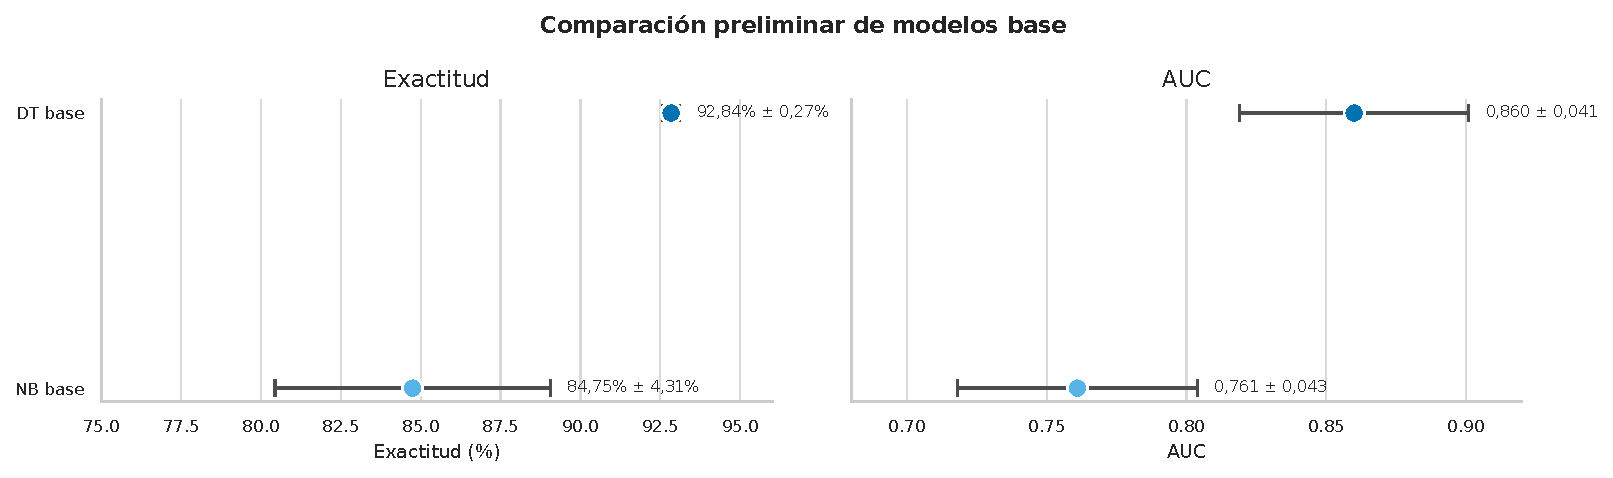
\includegraphics[width=0.94\textwidth]{output/figures/comparacion_modelos.pdf}
\caption{Comparación de exactitud y AUC para las cuatro variantes, con la variabilidad reportada por AI Studio.}
    \label{fig:model-comparison}
\end{figure}

\begin{figure}[H]
    \centering
    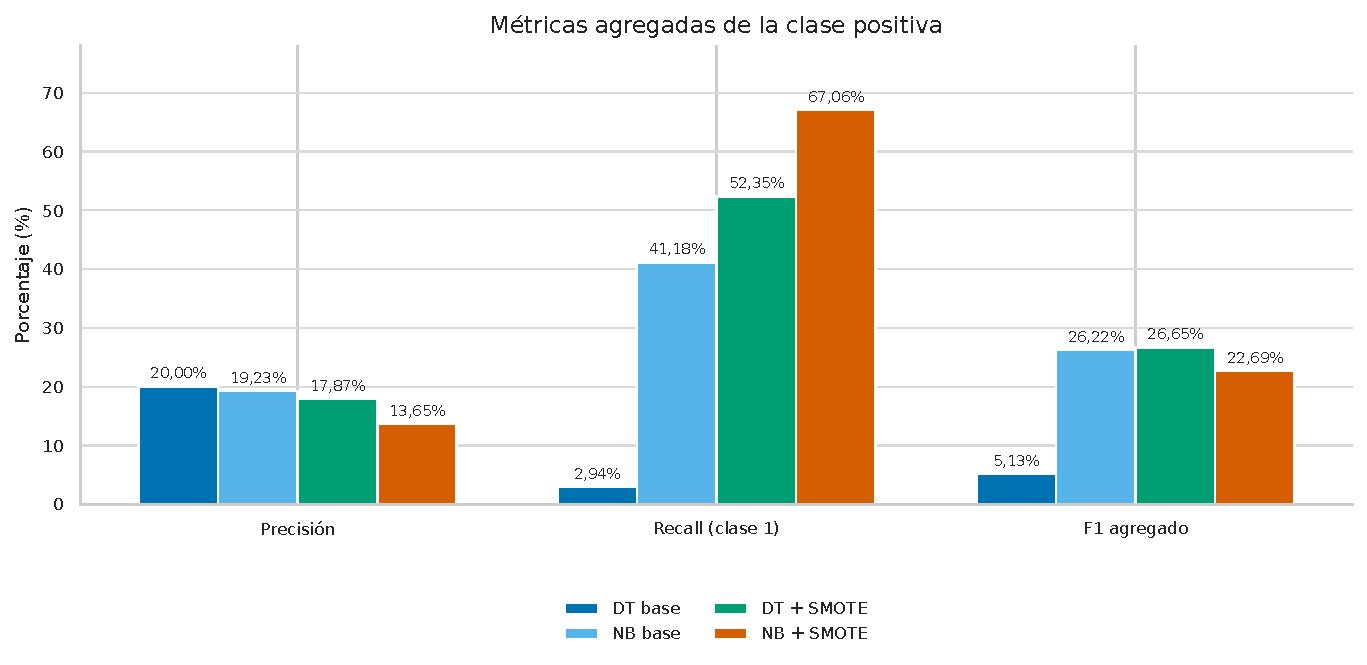
\includegraphics[width=0.94\textwidth]{output/figures/metricas_clase_positiva_cuatro_variantes.pdf}
    \caption{Precisión, recall y F1 agregados de la clase peligrosa para las cuatro variantes.}
    \label{fig:positive-metrics-comparison}
\end{figure}

\section{Discusión}

El árbol de decisión base conserva la exactitud y el AUC más altos, pero casi no detecta la clase 1: su recall agregado es 2,94\%. Este resultado confirma que, con una distribución donde la clase 0 representa 93,42\% de los registros, la exactitud aislada puede ocultar un comportamiento inadecuado para la detección de eventos peligrosos.

Naive Bayes con SMOTE maximiza el recall agregado de la clase 1, con 67,06\%, pero genera 721 falsos positivos. En consecuencia, aumenta la cobertura de eventos peligrosos a costa de una mayor cantidad de falsas alarmas, una exactitud menor y una precisión agregada de 13,65\%. El árbol de decisión con SMOTE ofrece un compromiso distinto: alcanza un recall agregado de 52,35\% con 409 falsos positivos y conserva un AUC de 0,824.

Entre estas cuatro variantes, el árbol de decisión con SMOTE presenta el mayor F1 agregado, 26,65\%. Este valor supera al de Naive Bayes base, 26,22\%, y al de Naive Bayes con SMOTE, 22,69\%. Por lo tanto, si el criterio combina precisión y recall mediante F1, DT + SMOTE es la variante más favorable en esta comparación. Si el objetivo prioritario es no omitir eventos peligrosos, NB + SMOTE resulta preferible por su recall, siempre que el sistema pueda gestionar el volumen de falsas alarmas.

La selección operativa no debe basarse en una única métrica. Debería incorporar una función de costos que asigne pesos explícitos a falsos negativos y falsos positivos, además de revisar la variabilidad entre particiones. Las conclusiones son válidas para la validación cruzada estratificada de 10 particiones informada y no reemplazan una evaluación temporal o una validación externa en condiciones de operación.

\section{Conclusiones y trabajo futuro}

La comparación muestra que el tratamiento del desbalance modifica sustancialmente el comportamiento de los clasificadores. SMOTE mejora la detección de la clase peligrosa en ambos algoritmos, pero reduce el rendimiento global y puede incrementar las falsas alarmas. En el conjunto analizado, DT + SMOTE logra el mayor F1 agregado, mientras que NB + SMOTE logra el mayor recall.

Como trabajo futuro se propone ajustar los hiperparámetros, calibrar los umbrales de decisión, estudiar una función de costos específica del contexto minero y evaluar la estabilidad temporal de los modelos en datos no utilizados durante el desarrollo.

\section{Referencia del conjunto de datos}

Sikora, M., y Wrobel, L. (2010). \textit{Seismic-Bumps}. UCI Machine Learning Repository.\\
\url{https://archive.ics.uci.edu/dataset/266/seismic+bumps}

\end{document}
